\documentclass{standalone}
\usepackage{tikz}
\usetikzlibrary{shapes, backgrounds}
\begin{document}
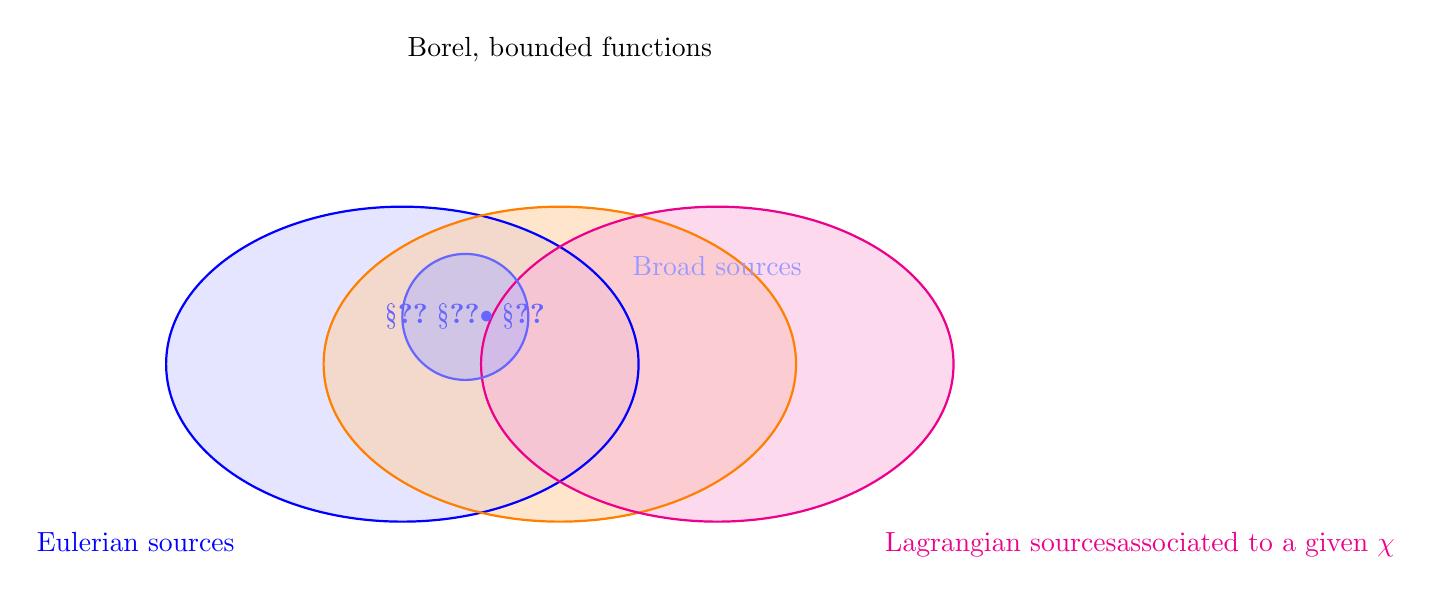
\begin{tikzpicture}
    \def\firstcircle{(0,0) ellipse (3cm and 2cm)}
    \def\secondcircle{(0:2cm) ellipse (3cm and 2cm)}
    \def\thirdcircle{(0:4cm) ellipse (3cm and 2cm)}

    \begin{scope}[fill opacity=0.5]
        \fill[blue!20] \firstcircle;
        \fill[orange!40] \secondcircle; % Note: This circle isn't visible as a separate entity but overlaps
        \fill[magenta!30] \thirdcircle;
        \fill[blue!30] (0.8,0.6) circle (0.8);
    \end{scope}

    \draw[blue, thick] \firstcircle node[below left=2cm] {\textcolor{blue}{Eulerian sources}};
    \draw[orange, thick] \secondcircle; % This is kept for structure but less visible
    \draw[magenta, thick] \thirdcircle node[below right=2cm] {\textcolor{magenta}{Lagrangian sources \\ associated to a given $\chi$}};
    \draw[blue!60, thick] (0.8,0.6) circle (0.8) node[] {\textcolor{blue!60}{\textsection\ref{s:L1} \textsection\ref{s:bound} \\ $\bullet$ \textsection\ref{s:Linfty}}};
    \node at (4, 1.25) {\textcolor{blue!40}{Broad sources}};

    \node at (2, 4) {Borel, bounded functions};
\end{tikzpicture}
\end{document}